% Tik output from JumanG
\documentclass{article}
\usepackage{tikz}
\pagestyle{empty}
\usepackage{verbatim}
\begin{document}
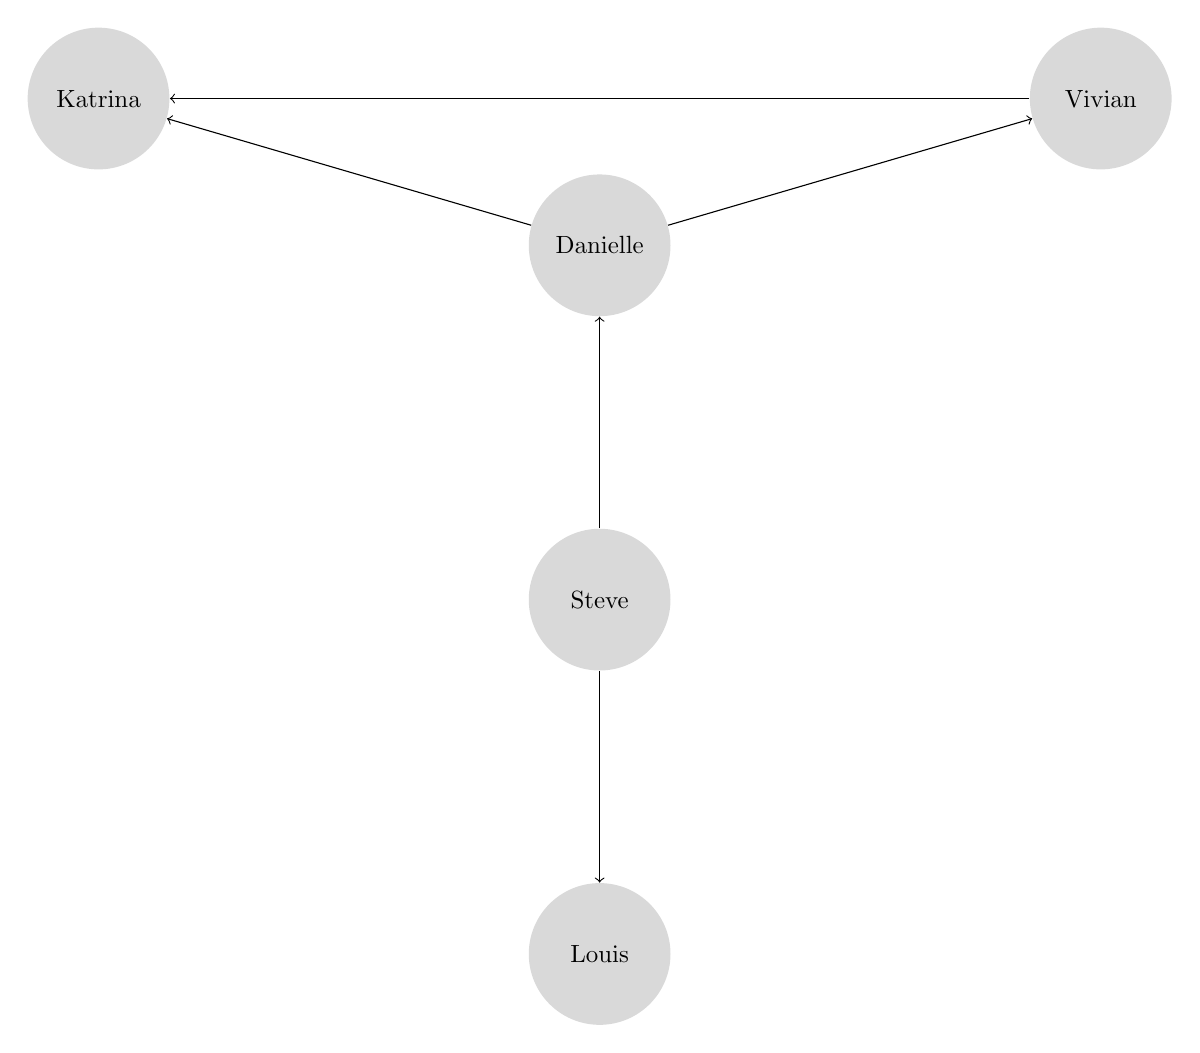
\begin{tikzpicture}[scale=.9, transform shape]
	\tikzstyle{every node} = [circle, fill=gray!30, minimum size = 2cm]
	\node (Steve) at (0, 0) {Steve};
	\node (Louis) at (0.0, -5.0) {Louis};
	\node (Katrina) at (-7.07106781187, 7.07106781187) {Katrina};
	\node (Danielle) at (0.0, 5.0) {Danielle};
	\node (Vivian) at (7.07106781187, 7.07106781187) {Vivian};
	\draw [->] (Steve)--(Danielle);
	\draw [->] (Steve)--(Louis);
	\draw [->] (Danielle)--(Vivian);
	\draw [->] (Danielle)--(Katrina);
	\draw [->] (Vivian)--(Katrina);
\end{tikzpicture}
\end{document}
